\documentclass{article}

\pdfoutput=1

\usepackage{amsmath}
\usepackage{amsfonts}
\usepackage{mathtools}
\usepackage{algorithm}
\usepackage{algorithmicx}
\usepackage{algpseudocodex}
\usepackage{graphicx}
\usepackage[margin=1in]{geometry}

\graphicspath{{figures/}}

\title{A Tool for Visualizing and Analyzing High-Dimensional Clustering Performance}
\author{Justin Lin\footnote{Department of Mathematics, Indiana University} and Julia Fukuyama\footnote{Department of Statistics, Indiana University}}
\date{}

\begin{document}
\maketitle

\abstract{Technological advances have spurred an increase in data complexity and dimensionality. We are now in an era in which data sets containing thousands of features are commonplace. To digest and analyze such high-dimensional data, dimension reduction techniques have been developed and advanced along with computational power. Of these techniques, nonlinear methods are most commonly employed because of their ability to construct visually interpretable embeddings. Unlike linear methods, these methods unevenly stretch and shrink space to create a visual impression that reflects the structure of the high-dimensional data. Unfortunately, capturing high-dimensional structures in a significantly lower number of dimensions requires drastic manipulation of space. As such, nonlinear dimension reduction methods are known to occasionally create false structures, especially in noisy settings. In efforts to deal with this phenomenon, we developed an interactive tool that enables analysts to better understand and diagnose their dimension reduction results. It uses various analytical plots to provide a multi-faceted perspective on captured structures in the data to determine if they're faithful or consquences of the dimension reduction process. The tool is available in an R package named \textit{DRtool}.}

\section{Introduction}
The potency of nonlinear dimension reduction methods lies in their flexibility, allowing them to model complex data structures. That same flexibility, however, makes them difficult to use and interpret. Each method requires a slew of hyperparameters that need to be calibrated, and even when adequately calibrated, these methods require a trained eye to interpret. For example, the two most popular nonlinear dimension reduction methods, t-SNE and UMAP, are known to generate unintuitive results (\cite{understanding UMAP}, \cite{Distill}). The results often cluster, even when no clusters exist in the data, and cluster sizes/placements can be unreliable. We've developed an interactive tool that analysts may use to conduct a post-hoc analysis of their high-dimensional clustering. The tool uses the minimum spanning tree (MST) to model the global structure of clusters and provide an additional perspective on inter-cluster relationships. This allows analysts to extract more information from their dimension reduction results by making it easier to differentiate the signal and the noise.

\section{Methods}

\subsection{The Minimum Spanning Tree}
Graphs have been applied to many multivariate statistical problems. The authors of \cite{MAP test} introduced the minimal ascending path spanning tree as a way to test for multimodality. The Friedman-Rafsky test \cite{Friedman-Rafsky test}, along with its modern variations \cite{Friedman-Rafsky variation 1, Friedman-Rafsky variation 2, Friedman-Rafsky variation 3}, use the MST to construct a multivariate two-sample test. Single-linkage clustering \cite{single-linkage and MST} and runt pruning \cite{runt pruning} are both intimately related with the MST. In the context of dimension reduction, IsoMap \cite{IsoMap} makes use of neighborhood graphs, \cite{MIST example} introduces the maximum information spanning tree, and \cite{MST example} uses the MST. These methods, which fall under the category of manifold learning, use graphs to model high-dimensional data assumed to be drawn uniformly from a high-dimensional manifold. An accurate low-dimensional embedding can then be constructed from these graphs. It's apparent that graphs are useful for modeling high-dimensional data, especially when it comes to dimension reduction and cluster analysis. Our tool uses the MST to analyze the reliability of visualizations produced by nonlinear dimension reduction methods.

We've opted for the MST for a couple of key properties. Firstly, the MST and shortest paths along it are quick to compute. Secondly, the MST contains a unique path between any two vertices, providing a well-defined metric on the data. Lastly, it provides a good summary of the data's structure. It contains as a subgraph the nearest-neighbor graph, and any edge deletion in the MST partitions the vertices into two sets for which the deleted edge is the shortest distance between them \cite{Friedman-Rafsky test}.

\subsubsection{MST Stability}
The MST is meant to provide a robust estimation of the data's global structure, and more specifically, inter-cluster relationships. As such, it should be stable in the presence of noise and unaffected by local transformations of the data. To demonstrate MST stability, we study the effect of random noise on the inter-cluster relationships explained by the MST.

To derive the inter-cluster relationships from the MST, we simplified the medoid subtree using the following procedure:

\begin{algorithm}[H]
\caption{Simplified Medoid Subtree}\label{algo1}
\begin{algorithmic}[1]
\Require MST $T = (V, E)$ with cluster medoids $m_1, \hdots, m_k \in V$
\State $T' = (V', E') \Leftarrow$ minimal subtree of $T$ containing all $m_i$
\Repeat
	\State Let $v \in V'$ with $deg(v) = 2$ and neighbors $a, b \in V'$. Let $d(v, a)$ and $d(v, b)$ be the weights of the edges connected $v$ and to $a$ and $b$.
	\State Replace $v$ and its two incident edges with an edge connecting $a$ and $b$ with weight $d(v, a)$ and $d(v, b)$.
\Until{$T'$ contains no longer contains non-medoid vertices with degree two}
\State \Output T'
\end{algorithmic}
\end{algorithm}

The simplification process essentially replaces paths of non-medoid vertices with one edge of equal length. We refer to this tree as the simplified medoid subtree. It encode global inter-cluster relationships within the data.

\subsubsection{Robinson-Foulds Metric}
To compare simplified medoid subtrees, we used the Robinson-Foulds metric \cite{RF metric}. The R-F metric was originally introduced to quantify the dissimilarity of phylogenetic trees, but the algorithm generalizes to arbitrary weighted trees. It looks at partitions of each tree created by removing individual edges, then counts the number of partitions present in one tree but not in the other. We modified the algorithm (Algorithm 2) to specifically measure the dissimilarity in medoid vertices and applied a normalization so that the distances range from zero to one.

\begin{algorithm}[H]
\caption{Robinson-Foulds Distance}\label{algo2}
\begin{algorithmic}[2]
\Require Trees $T_1 = (V_1,E_1)$ and $T_2 = (V_2, E_2)$ with medoids $m_1, \hdots, m_k \in V_1$ and $n_1, \hdots, n_k \in V_2$
\State $P_1 \Leftarrow \{\}$
\For{$e \in E_1$}
	\State $G \Leftarrow (V_1, E_1 \setminus \{e\})$ with connected components $G_1$ and $G_2$
	\State $M_1 \Leftarrow \{m_1,\hdots,m_k\} \cap V(G_1)$
	\State $M_2 \Leftarrow \{m_1,\hdots,m_k\} \cap V(G_2)$
	\State $P_1 \Leftarrow \Call{Add}{P_1, \{M_1, M_2\}}$
\EndFor
\State $P_2 \Leftarrow \{\}$
\For{$e \in E_2$}
	\State $G \Leftarrow (V_2, E_2 \setminus \{e\})$ with connected components $G_1$ and $G_2$
	\State $M_1 \Leftarrow \{n_1,\hdots,n_k\} \cap V(G_1)$
	\State $M_2 \Leftarrow \{n_1,\hdots,n_k\} \cap V(G_2)$
	\State $P_2 \Leftarrow \Call{Add}{P_2, \{M_1, M_2\}}$
\EndFor
\State \Output $\frac{\left|P_1 \Delta P_2 \right|}{2\left| P_1 \cap P_2 \right|}$
\end{algorithmic}
\end{algorithm}

\subsection{The PCA -- CCA Method}
To understand the relationship between two specific clusters, the tool requires the user to specify a path connecting said clusters. Once a path is specified, a local projection method is applied to visualize the path and nearby points of interest in two dimensions.

Let $P \in \mathbb{R}^{k \times p}$ be the matrix of high-dimensional path points with endpoints $p_1, p_k \in \mathbb{R}^p$. Let $X \in \mathbb{R}^{n \times p}$ be the matrix of points of with interest. By default, the points of interest include the path points and all points belonging to the same cluster as $p_1$ or $p_k$. Alternatively, the user may select point there own points of interest.

The idea is to use canonical-correlation analysis (CCA) to determine the two-dimensional projection that best unwinds the path. Given two data matrices with an equal number of rows, CCA iteratively calculates linear combinations of the matrix features, known as canonical variate pairs, that maximize covariance. The canonical variate pairs are chosen to be orthogonal to all previous pairs, so they give rise to a projection subspace. To unwind $P$, we use CCA to compare P against the data matrix modeling a $d$-dimensional polynomial $$P_d = \begin{bmatrix}
1 & 1^2 & \cdots & 1^d \\
2 & 2^2 & \cdots & 2^d \\
\vdots & \vdots & & \vdots \\
n & n^2 & \cdots & n^d
\end{bmatrix}$$
and use the first two canonical variate pairs to construct a two-dimensional projection of $P$ that maximizes its covariance with $P_d$

\section{Results}

\subsection{MST Stability Experiment}
1,500 samples were randomly chosen from the MNIST data set \cite{MNIST}. Each $784 \times 784$-pixel image was flattened into a vector of length $784^2$, so the data contain 1,500 samples in $784^2$ dimensions. A PCA pre-processing step was employed to reduce the number of dimensions to 300. The simplified medoid subtree $T$ was then calculated.

Random Gaussian noise was then added to the data and the new simplified medoid subtree $T'$ was calculated. The R-F distance $RF(T, T')$ was recorded. This process was repeated 30 times.

\renewcommand{\figurename}{Figure}
\renewcommand{\thefigure}{1}
\begin{figure*}[!b]
\centering
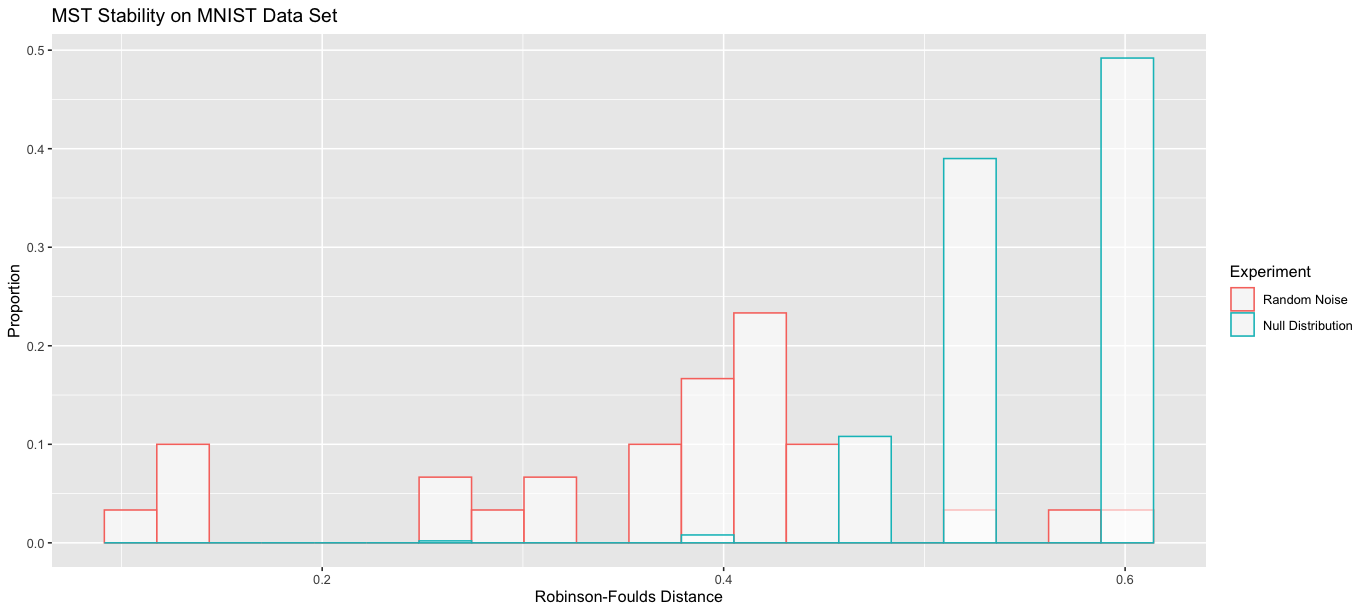
\includegraphics[scale=0.3]{RF stability}
\caption{MST Stability on MNIST Data Set}
\end{figure*}

To better interpret the R-F distances, we designed a null distribution of distances as a reference for comparison. These distances should represent R-F distances between trees that do not portray similar global structures and inter-cluster relationships. To generate the null distribution from the data, we randomly permuted the class labels and computed the R-F distances between the resulting simplified medoid subtrees and the original simplified medoid subtree. By randomly re-labelling the clusters, we are simulating examples with distinct global structures. Figure 1 shows the R-F distances produced by adding noise and permuting the class labels. The simplified medoid subtree trees generated by adding noise were significantly closer to the original simplified medoid subtree than those generated by randomly permuting the class labels in terms of R-F distance.

\newpage

\begin{thebibliography}{10}

\bibitem{fractional Lp norms}
Charu C. Aggarwal, Alexander Hinneburg, and Daniel A. Keim.
\newblock On the surprising behavior of distance metrics in high dimensional space.
\newblock {\em Lecture Notes in Computer Science, vol. 1973}, 2001.

\bibitem{Friedman-Rafsky variation 1}
Bhaswar B. Bhattacharya.
\newblock A general asymptotic framework for distribution-free graph-based two-sample tests.
\newblock {\em Journal of the Royal Statistical Society Series B: Statistical Methodology 81:3, 575-602}, 2019.

\bibitem{Friedman-Rafsky variation 2}
Hao Chen and Jerome H. Friedman.
\newblock A new graph-based two-sample test for multivariate and object data.
\newblock {\em Journal of the American Statistical Association 112:517, 397-409}, 2017.

\bibitem{Friedman-Rafsky variation 3}
Hao Chen, Xu Chen, and Yi Su.
\newblock A weighted edge-count two-sample test for multivariate and object data.
\newblock {\em Journal of the American Statistical Association 113:523, 1146-1155}, 2018.

\bibitem{understanding UMAP}
Andy Coenen and Adam Pearce for Google PAIR.
\newblock Understanding UMAP.
\newblock {\em https://pair-code.github.io/understanding-umap/}.

\bibitem{MNIST}
Li Deng.
\newblock The MNIST database of handwritten digit images for machine learning research.
\newblock {\em IEEE Signal Processing Magazine 29:6}, 2012.

\bibitem{image metrics}
Vito Di Ges\`u and Valery Starovoitov.
\newblock Distance-based functions for image comparison.
\newblock {\em Pattern Recognition Letters 20:2, 207-214}, 1999

\bibitem{single-linkage and MST}
J. C. Gower and G. J. S. Ross.
\newblock Minimum spanning trees and single linkage cluster analysis.
\newblock {\em Journal of the Royal Statistical Society. Series C (Applied Statistics) 18:1, 54-64}, 1969.

\bibitem{Friedman-Rafsky test}
Jerome H. Friedman and Lawrence C. Rafsky.
\newblock Multivariate generalizations of the Wald-Wolfowitz and Smirnov two-sample tests.
\newblock {\em Annals of Statistics 7:4, 697-717}, 1979.

\bibitem{MIST example}
Bracken M. King and Bruce Tidor.
\newblock MIST: Maximum information spanning trees for dimension reduction of biological data sets.
\newblock {\em Bioinformatics 25:9, 1165-1172}, 2009.

\bibitem{text data}
Abdul Wahab Qurashi, Violeta Holmes, and Anju P. Johnson.
\newblock Document processing: Methods for semantic text similarity analysis.
\newblock {\em IEEE}, 2020.

\bibitem{runt pruning}
Werner Stuetzle.
\newblock Estimating the cluster tree of a density by analyzing the minimal spanning tree of a sample.
\newblock {\em Journal of Classification 20, 25-47}, 2003.

\bibitem{IsoMap}
Joshua B. Tenenbaum, Vin de Silva, and John C. Langford.
\newblock A global geometric framework for nonlinear dimensionality reduction.
\newblock {\em Science 290:2319}, 2000.

\bibitem{MST example}
Daniel Probst and Jean-Louis Reymond.
\newblock Visualization of very large high-dimensional data sets as minimum spanning trees.
\newblock {\em Journal of Cheminformatics 12:12}, 2020.

\bibitem{MAP test}
Gregory Paul M. Roz\'al and J.A. Hartigan.
\newblock The MAP test for multimodality.
\newblock {\em Journal of Classification 11, 5-36}, 1994.

\bibitem{RF metric}
D. F. Robinson and L. R. Foulds.
\newblock Comparison of Phylogenetic Trees.
\newblock {\em Mathematical Biosciences 53, 131-147}, 1981.

\bibitem{Distill}
Martin Wattenberg, Fernanda Vi\'egas, and Ian Johnson.
\newblock How to Use t-SNE Effectively.
\newblock {\em Distill}, 2016.

\end{thebibliography}

\end{document}